\chapter{Grundlagen}
Um die Inhalte wie Konzeption und Implementierung aber auch verwandte Arbeiten nachvollziehen zu können, werden in diesem Kapitel grundlegende Begriffe, Techniken sowie Technologien erläutert.

\section{Definitionen}
    \subsection{Smart Devices} \label{SmartDevices}
        \glqq informationstechnisch [sic] aufgerüstete Alltagsgegenstände, die einen Mehrwert durch sensorgestützte Informationsverarbeitung und Kommunikation erhalten.\grqq{} \cite{lackes_siepermann_2018}
        
        Dieses Zitat von Herr Lakes et al. nennt als Hauptmerkmale eines solchen Geräts den alltäglichen Einsatz der Gegenstände, welche mithilfe von Sensorik und Kommunikation einen Mehrwert generieren.
        Nimmt man nun ein Gerät, welches als \emph{Smart Device} bezeichnet wird, erkennt man, dass die Aussage zutreffend ist. Als Beispiel lässt sich eine intelligente Steckdose heranziehen. Sie ist ein alltäglicher Gegenstand, welcher über Funk angesteuert werden kann. Somit kann ein anderes Gerät, welches sich mit der Steckdose verbinden lässt, den aktuellen Status abfragen oder verändern.
        Der Funk, welcher in normalen Steckdosen nicht verfügbar ist, und übermittelt den aktuellen Status an ein externes Gerät. Mithilfe dieses Gerätes ist dann eine Steuerung der Steckdose möglich, was einen Mehrwert bietet.
    
    \subsection{Internet der Dinge}
        \glqq bezeichnet [sic] die Vernetzung von Gegenständen mit dem Internet, damit diese Gegenstände selbstständig über das Internet kommunizieren und so verschiedene Aufgaben für den Besitzer erledigen können. Der Anwendungsbereich erstreckt sich dabei von einer allg. Informationsversorgung über automatische Bestellungen bis hin zu Warn- und Notfallfunktionen.\grqq{}
        \cite{lackes_siepermann_2018_iot}.
    
        Die Definition des Begriffs \emph{Internet der Dinge} oder \ac{IoT} von Herr Lakes et al. deckt sich in vielen Punkten mit der Definition \ref{SmartDevices}. Hier befinden sich ebenfalls vernetzte Geräte, welche sich untereinander mit Informationen versorgen und somit Aufgaben übernehmen (also einen Mehrwert bieten) können. Das Wichtige an diesem Begriff ist der Zusammenschluss solch intelligenter Geräte in größere Netze. Die Geräte müssen dabei nicht gleichartig sein und können unterschiedliche Aufgaben im Alltag übernehmen. Sie können Abhängigkeiten zueinander besitzen und sich gegenseitig Ansprechen oder aktivieren ohne direkte Befehle vom Besitzer, also Nutzer, zu erhalten.
        
        Diese Vorstellung von \ac{IoT} teilt auch Ashton im RFID Journal.
        %http://www.itrco.jp/libraries/RFIDjournal-That%20Internet%20of%20Things%20Thing.pdf
        \glqq If we had computers that knew everything there was to know about things—using data they gathered without any help from us—we would be able to track and count everything, and greatly reduce waste, loss and cost. We would know when things needed replacing, repairing or recalling, and whether they were fresh or past their best.\grqq{} \cite{ashton2009internet}
        Dieses Zitat beschreibt die Motivation, welche hinter dem \emph{Internet der Dinge} steht.
        Im Fokus ist die Automatisierung von Abläufen, ohne Zutun von Menschen. Darüber hinaus bekommen Menschen umfassende Informationen über aktuelle Zustände aller Geräte und können ihre Aktionen besser koordinieren. Dies würde die Abläufe effizienter machen, wodurch Geld eingespart und Prozesse optimiert werden können.

\section{MQTT}
    \subsection{Publish/Subscribe}
    Das publish/subscribe-Prinzip besteht aus einer Client-Server-Architektur, wobei nur der Client aktiv kommuniziert. Der Broker ist eine Endstelle, welche meist vom Betreiber zur Verfügung gestellt wird und die Nachrichten empfängt und bei sich veröffentlicht. Der Client verbindet sich mit dem Broker und hält eine Verbindung zu diesem offen, wodurch er die Nachrichten an eine sogenannte Topic, vergleichbar mit einem Postfach im Broker, sendet. Gleichzeitig kann er mehrere angelegte Topics abonnieren (oder auch  \glqq subscriben\grqq{} genannt), was bedeutet, dass er in diesem Pfad auf neuen Nachrichten wartet. Sobald sie beim Broker eintrifft, veröffentlicht er diese für die Clients. Anschließend können diese die Informationen der Mitteilungen verarbeiten. \cite{Redbooks2012}

    Dieses Prinzip ermöglicht eine Kommunikation zwischen Geräten, welche keine stabile Verbindung besitzen oder eine niedrige Bandbreite einhalten müssen. Im Gegensatz zu dem Request/Response-Prinzip, welches unter anderem bei Webseiten verwendet wird, ist es hier nicht nötig sogenannte \glqq Update-Requests\grqq{} zu senden, da die Verbindung offen gehalten wird.
    Diese Eigenschaft eignet sich besonders für \emph{Smart Devices}, die wenig Rechenkraft besitzen oder die nur wenig Informationen bei Bedarf senden müssen. \cite{Hwang2016}

    \subsection{Standard}
        \ac{MQTT} ist ein Protokoll, welches auf dem zuvor beschriebenen Publish/Subscribe-Prinzip basiert. Es wurde ursprünglich zwischen 1998 und 1999 von IBM und Arcom (heute Eurotech) entwickelt. Die Version 3.1.1 wurde Ende 2014 von der OASIS Foundation als Standard verabschiedet und ist bis heute noch der De-Facto-Standard. Dies ist ebenfalls anhand des ISO/IEC Standards zu erkennen, worin das Protokoll in 2016 unter der Bezeichnung 20922 aufgenommen wurde \cite{eclipse_foundation2017}. Mitte 2019 wurde die MQTT-Version 5.0 ebenfalls als OASIS Standard verabschiedet. Anhand von weiteren Funktionen und Rückwärtskompatibilität wird sichergestellt, dass zukünftige Geräte besser unterstützt werden können. \cite{mqtt_org_2019}.
        
        \ac{MQTT} ist ein sehr kompaktes Protokoll, mit dem Zweck der \ac{M2M} Kommunikation.
        Es setzt auf \ac{TCP} auf und arbeitet asynchron\footnote{Das heißt es werden mehrere Anfragen parallel verarbeitet, anstatt auf den Abschluss der vorigen zu warten} nach dem publish/subscribe-Prinzip. Es existieren im einfachsten Fall zwei Akteure. Der Broker (alternativ auch \glqq Server\grqq{} genannt), welcher die Topics enthält und der Client, der Nachrichten an Topics sendet und weitere abonniert.
        Um garantieren zu können, dass die Nachrichten auch ankommen gibt es die Möglichkeit ein \ac{QoS} zu definieren. Um dem gewünschten Szenario zu entsprechen, existieren drei verschiedene Stufen. 
        \cite{soni2017survey}
        \begin{itemize}
            \item \glqq QoS 0: At most once delivery\grqq{}: Es wird keine Antwort vom Empfänger gesendet und die Nachricht wird nicht erneut versendet. Entweder wird die Nachricht beim ersten Mal empfangen oder nie.
            \item \glqq QoS 1: At least once delivery\grqq{}: Es wird eine Antwort vom Empfänger erwartet. Bleibt diese aus, wird die Nachricht erneut versendet, bis der Sender eine Antwort erhält.
            \item \glqq QoS 2: Exactly once delivery\grqq{}: Dies ist die höchste Qualitätsstufe und garantiert, dass die Nachricht an der Endstelle sicher ankommt und zusätzlich dazu auch nur einmal empfangen werden kann, also keine Duplikate entstehen. Um dies zu erreichen, ist es jedoch notwendig die Pakete des leichtgewichtigen Protokolls mit weiteren Daten anzureichern was zu einem erhöhten Größe und somit größerem Aufwand führt.
        \end{itemize} \cite{gupta_banks_2015}
        Obwohl \ac{MQTT} auf \ac{TCP} basiert, wurde es so entworfen, dass es im Vergleich zu alternativen Protokollen nur das Nötigste enthält. \cite{soni2017survey}

    \subsection{Sicherheit}
        Das Protokoll V3.1 und höher kann im Standard nur mit einem Benutzernamen und Passwort gesichert werden. Eine Transportverschlüsselung ist mithilfe von \ac{TLS}/\ac{SSL}, welche auch im Sicherheitsprotokoll für \ac{HTTP} (auch \ac{HTTPS} genannt) verwendet werden um das Internet zu sichern, als zusätzliche Maßnahme möglich. Jedoch beinhaltet SSL viele Informationen, welche in Bezug auf \ac{MQTT} nicht notwendig sind und somit die Paketegröße unverhältnismäßig erhöht.
        Dies kann sich in verschiedenen Szenarien als problematisch herausstellen, da \ac{MQTT} genau für das Gegenteil nämlich der sparsamen Kommunikation, entwickelt wurde.
        Eine Alternative oder zusätzliche Maßnahme zum Schützen der Inhalte ist eine anwendungsbasierte Verschlüsselung der übertragenen Daten. Dies muss jedoch unabhängig vom Protokoll vom Hersteller implementiert werden, wodurch weitere Sicherheitsrisiken (wie zum Beispiel fehlerhafte Kryptographie) entstehen können. \cite{mqtt_org_2019}.

    \subsection{Produkte}
        Es gibt verschiedene Anbieter, die Bibliotheken aus dem Standard entwickelt haben. Auch wenn sie den gleichen Standard implementieren, haben Sie verschiedene Schwerpunkte und somit Unterschiede. Einer der bekanntesten Broker ist die quelloffene Implementierung Eclipse Mosquitto \cite{eclipse_foundation_inc_2018}. Darüber hinaus gibt noch weitere Dienstleister, welche komplette Services um das Verwalten und Steuern von Broker bereitstellen. Bekannte Vertreter sind HIVEMQ \cite{hivemq_dc_square_gmbh} und CloudMQTT \cite{84codes_ab_2019}.
        %More information about the protocol can be found on the MQTT.org community site.

\section{Technologien}
        \subsection{Zertifikate}
        Siller beschreibt Zertifikate wie folgt:
        \glqq Ein digitales Zertifikat ist ein digitaler Datensatz, der bestimmte Eigenschaften von Personen oder Objekten bestätigt und dessen Authentizität und Integrität durch kryptografische Verfahren geprüft werden kann.\grqq{} \cite{siller_2018}.
        Um Personen oder Objekte identifizieren zu können, muss im ersten Schritt eine Endstelle sicherstellen und prüfen, dass die eingegeben Daten der Wahrheit entsprechen. So eine Endstelle wird auch TrustCenter (oder auch \glqq \ac{CA}\grqq{} genannt) bezeichnet und repräsentiert eine ausgewählte, vertrauenswürdige dritte Organisation. Nach der Verifikation aller erforderlichen Daten, wird das digitale Zertifikat ausgestellt und den Nutzern oder Endgeräten zur Verfügung gestellt. Mithilfe der Informationen aus den Zertifikaten kann das Endgerät anschließend eine passende Verbindung aufbauen und gleichzeitig sicherstellen, das die Verbindung auch mit dem im Zertifikat definierten Endpunkt hergestellt wird.
    
    \subsection{.NET Framework}
        Das .NET Framework ist nach Thai et al. ein Framework, das eine Schnittstelle zu Windows-Diensten und weiteren Windows-Funktionalitäten darstellt \cite{thai2003net}.
        Unterstützte Sprachen (unter anderem C\# und Visual Basic.NET) werden im Laufe der Kompilierung in Bytecode umgewandelt. Erst zur Laufzeit wird dieser in Maschinencode übersetzt und anschließend ausgeführt. Es existieren zahlreiche Implementierungen von Basisfunktionalitäten (z.B. Zugriff auf das Dateisystem) und komplexen Funktionalitäten wie dem Zugriff auf verteilte Systeme. 
        Das \emph{Assemblysystem} des .NET Framework ermöglicht das Auslagern von Funktionalitäten in Bibliotheken und die Wiederverwendung von diesen.
        
    \subsubsection{Mono für Plattformunabhängigkeit}
        Um eine plattformunabhängige Verwendung der Programme zu ermöglichen, wurde Mono entwickelt.
        Wie der offiziellen Webseite \cite{mono_project_2018} zu entnehmen ist, ist Mono eine Entwicklungsplattform auf Basis des .NET Frameworks von Microsoft und stellt dessen Funktionalität auf verschiedenen Plattformen zur Verfügung. Um die Funktionalität abbilden zu können, besteht Mono aus verschiedenen Komponenten.
        Der C\#-Kompiler beinhaltet alle genormten Funktionen der C\#-Versionen 1.0 - 6.0.
        Die Laufzeitumgebung beinhaltet neben zwei Kompilern auch eine Möglichkeit zum Laden von Bibliotheken sowie zum parallelen Ausführen von Anwendungen und einen Garbage-Collector.
        Die Mono-Implementierung der .NET Framework Standardbibliotheken ist kompatibel mit denen von Microsoft.
        Monos Standardbibliotheken stellen darüber hinaus noch weitere Zusatzfunktionalitäten zur Verfügung, die entweder plattformabhängig sind oder nützliche Zusätze wie Verarbeiten von Zip-Archiven oder Anbindung an Authentifizierungssysteme sind.

\section{Konzepte}
    \subsection{Proxy}
    Die Oxford University Press definiert Proxy als \glqq A person authorized to act on behalf of another.\grqq{} und beschreibt somit das Wort im normalen Sprachegebrauch \cite{oxford_university_press_2019}.
    Tauscht man den Begriff \glqq Person\grqq{} durch \glqq Gerät\grqq{}, bekommt man eine passende technische Definition. Es handelt sich bei einem technischen Proxy um ein Gerät das im Namen eines anderen Gerätes handelt.

    \subsection{Man In The Middle}
        Im Szenario, welches in Abbildung \ref{fig:szenario-mitm} dargestellt wird, versucht sich die Lampe (in diesem Beispiel der Client) mit dem Broker von \glqq my.broker.com\grqq{} zu verbinden. Diese Verbindung würde im Normalfall direkt und ohne Umweg aufgebaut werden um Daten auszutauschen. Mithilfe verschiedener Methoden ist es jedoch möglich den Datenfluss, wie in der Abbildung dargestellt, zu verändern.
        \subsubsection{DNS}
        Mithilfe von Einträgen im \ac{DNS} in der Firewall oder einem Router ist es möglich die \ac{DNS}-Anfragen\footnote{Ein Client fragt nach der \acs{IP}-Adresse des Gerätes (z.B.: google.de -> 216.58.207.35)} manuell zu überschreiben. Somit wird beim Aufruf des Brokers nicht die originale (oder auch externe) IP-Adresse\footnote{Die \acs{IP}-Adresse identifiziert jedes Gerät in einem Netzwerk eindeutig und ermöglicht das Verteilen von Paketen über Netzwerke hinweg.}, sondern die überschriebene zur Verfügung gestellt.
        \subsubsection{ARP}
        Durch das \ac{ARP} können Einträge im \ac{DNS} von extern verändert werden. Mithilfe des sogenannten \ac{ARP}-poisoning Angriffs werden Pakete einer veränderten \ac{MAC}-Adresse (die des Opfers) an die legitimen \ac{ARP}-Anfragen gesendet. Dies ist möglich, da diese Anfragen an alle Teilnehmer in einem Netzwerk gesendet werden und die am schnellsten antwortende Nachricht akzeptiert wird. Dies verändert die Korrelation der \acs{IP}-Adresse zur \acs{MAC}-Adresse, was dazu führt, dass Nachrichten für das Opfer an den Angreifer gesendet werden. \cite{4768661}
        \subsubsection{ICMP}
        Durch das \ac{ICMP} ist es möglich, mithilfe einer Nachricht zur Weiterleitung von Paketen, den Nachrichtenfluss über das eigene Gerät laufen zu lassen.
        Diese Nachricht wird üblicherweise dazu verwendet, Router über einen besseren bzw. schnelleren Weg zu informieren, jedoch kann sie auch manuell erzeugt und somit missbraucht werden. Obwohl diese Methode den großen Vorteil bietet, nicht im lokalen Netz sein zu müssen, ist der Nachteil, dass viele Router statische Routen verwenden oder diese Pakete schlichtweg abweisen, nicht zu ignorieren.
        \subsubsection{Firewall}
        Die Firewall möglich es, das Netzwerk des Clients vom Netzwerk des Brokers zu trennen. Anschließend kann dank der Portweiterleitung eine Regel angelegt werden, die Nachrichten aus dem \ac{LAN} an ein beliebiges Gerät weiterleiten. Dies ist im Gegensatz zu den vorigen Methoden sehr zuverlässig und performant, da keine unberechtigte Manipulation stattfindet und kein zusätzlicher Netzwerkverkehr generiert wird. Der Nachteil dieser Lösung ist jedoch, dass ein extra Gerät (in diesem Fall die Firewall) etabliert werden muss und alle Geräte, welche weitergeleitet werden sollen, an die \ac{LAN} Schnittstelle angeschlossen werden müssen.
        
        \begin{figure}[h]%h=direkt danach t=top b=bottom
            \centering
            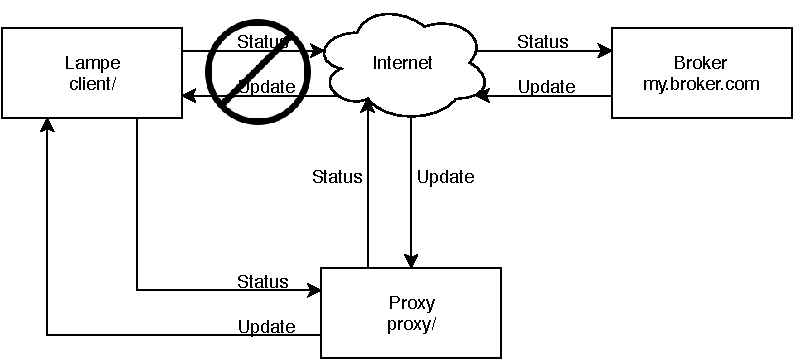
\includegraphics[width=14cm]{tex/bilder/2_grundlagen/Szenario1_MitM.pdf}
            \captionof{figure}{Darstellung eines Szenarios mit MITM}
            \label{fig:szenario-mitm}
        \end{figure}
        
    \subsection{Security Assessment}
        Um den Arbeitsablauf eines Penetrationtesters aufzuzeigen, werden die sieben Schritte des \ac{PTES} \cite{hsiangchih_2019} beschrieben.
    
    \subsubsection{\glqq Pre-engagement Interactions\grqq{}}
        Es werden alle Vorbereitungen und Absprachen zum Umfang, wie Zeit und \acs{IP}-Adressen, und Art des Tests (wie zum Beispiel Netzwerk-, Penetration-Test) besprochen.
    \subsubsection{\glqq Intelligence Gathering\grqq{}}
        Hier werden so viele Informationen über das Ziel herausgefunden wie nur möglich. Dies ist notwendig um ein bestmögliches Bild über das Ziel zu bekommen und sich viele Angriffsvektoren\footnote{Der Angriffsvektor ist die Methode, mit der ein Angriff sein Ziel erreicht \cite{HANSMAN200531}.} einfallen lassen kann. Dies ist außerdem essentiell, um Sicherheitsmaßnahmen im Vorhinein zu identifizieren, die umgangen werden sollten, um nicht sofort aufzufallen. Das reduziert die Aktionen, welche in Logdateien gespeichert werden und verschleiert die Anwesenheit des Angreifers. Als Beispiel ist es möglich eine Aktion mit zufällig generierten Werten aufzurufen. Dies würde allerdings eine Menge an fehlerhafter Anfragen dokumentieren, die offensichtlich nicht durch die Software auf Seite des Herstellers hervorgerufen wurden. Als Alternative ist es möglich die bestehende Kommunikation zu untersuchen und auf Basis der observierten Kommunikation vom Endgerät leicht abgewandelte Versionen zu erzeugen. Hierbei hilft die konzipierte Software als Alternative zu bestehenden Lösungen wie Wireshark\footnote{Wireshark, ein Tool zum Überwachen und Aufzeichnen des Netzwerkverkehrs \cite{SandersChris2017Ppa}}, um diese Kommunikation zu überwachen und Informationen über die Kommunikation zu erfassen.
    \subsubsection{\glqq Threat Modeling\grqq{}}
        Nachdem Informationen über den Dienst gesammelt wurden, ist der Tester nun in der Lage ein Modell zu entwickeln, in dem Services klassifiziert und anhand der Risiken Maßnahmen zur Milderung der Gefahr aufgenommen werden. Diese können, zum Beispiel bei nicht ausreichend geschützten Eingängen und Ausgaben, filtern von Sonderzeichen oder Plausibilitätprüfungen beinhalten.
    \subsubsection{\glqq Vulnerability Analysis\grqq{}}
        In diesem Schritt wird die Applikation auf Schwachstellen untersucht. 
        Dieser Schritt ist in zwei Teile, die Identifikation und die Prüfung, geteilt.
        Die Identifikation wird mithilfe von aktiven und passiven Methoden durchgeführt.
        Auf der einen Seite stehen Tools für aktive Tests wie zum Beispiel 
        SQLMap \cite{damele_stampar_2014}, 
        Burp Suite \cite{LozanoCarlosA.author2019Hapt}, %https://proquestcombo.safaribooksonline.com/book/web-development/9781788994064
        Nessus \cite{BealeJay2008Nna}, %https://proquestcombo.safaribooksonline.com/9781597492089
        \ac{ZAP} \cite{bennetts2013owasp}. %https://www.owasp.org/images/9/96/OWASP_2014_OWASP_ROMANIA.pdf
        Nachdem die Tools eingestellt sind, scannen und interagieren mit den Funktionalitäten der Seite oder Applikation ohne weitere Aktionen vom Nutzer.
        Auf der anderen Seite stehen die passiven Tools wie Wireshark oder TCPdump \cite{tcpdump_2010}, welche außenstehend sind und nur die Aktionen anderer aufzeichnen. 
        Diese gefundenen Schwachstellen werden anschließend verifiziert, also auf Korrektheit geprüft und zum Schluss anhand der Risiken aus Sicht der Applikation bewertet \cite{hayes_2012}.
    \subsubsection{\glqq Exploitation\grqq{}}
        In diesem Schritt wird versucht, unter Umgehen weiterer Sicherheitsmechanismen, die bestätigte Schwachstelle so zu verwenden, dass entweder eine Steigerung der Berechtigungen oder das weitere Infiltrieren erreicht wird.
    \subsubsection{\glqq Post Exploitation\grqq{}}
        Im vorletzten Schritt wird versucht den erlangten Zugriff zu festigen und eventuelle benötigte Daten herunterzuladen. Das heißt, dass selbst nach dem Neustart des Systems die Kontrolle über das System bestehen bleibt ohne erneut den Exploit zu verwenden. Üblicherweise wird dies mithilfe von einem \ac{RAT} gemacht, welche in den Autostart, die Registry geschrieben. Diese Programme ermöglichen die Steuerung des Computers ohne physischen Zugriff zu haben. Des Weiteren sind die Programme sehr gut versteckt, um nicht aufzufallen. Die Namen ähneln meist Dienst- oder Programmbezeichnungen, um legitim auszusehen. Es gibt ebenfalls die Möglichkeit, das Programm so zu schützen, dass beim Versuch das Programm zu beenden das System selbst herunterfährt.
    \subsubsection{\glqq Reporting\grqq{}}
        Dies ist der letzte und einer der wichtigsten Schritte. Da Security-Tests durchgeführt werden um die Sicherheit zu erhöhen, ist es auch zwingend notwendig die Schwachstellen und Exploits so zu dokumentieren, dass der Hersteller sich entscheiden kann, ob die existierenden Probleme behoben werden oder das Risiko getragen wird. Abhängig von dem Einfluss auf das Geschäft (auch \glqq Business Impact\grqq{} gennant) kann es aus wirtschaftlicher Sicht gerechtfertigt sein, eine Schwachstelle nicht zu schließen und die daraus resultierenden Folgen zu tragen, d.h. beispielsweise Geldstrafen zu zahlen.

\section{IoT Security}
    \subsection{OWASP IoT Guide}
        Die OWASP Foundation \cite{guzman_2019} beschreibt das \ac{OWASP} wie folgt.
        \glqq OWASP is an open community dedicated to enabling organizations to conceive, develop, acquire, operate, and maintain applications that can be trusted. All of the OWASP tools, documents, forums, and chapters are free and open to anyone interested in improving application security. We advocate approaching application security as a people, process, and technology problem because the most effective approaches to application security include improvements in all of these areas.\grqq{}
        
        Das bedeutet, dass das Projekt eine offene Gemeinschaft ist, welche freie und unentgeltlich nutzbare Software zum Testen von IT-Sicherheit bereitstellt. Darüber hinaus veröffentlichen sie ebenfalls jährliche Ranglisten bezüglich der am häufigsten vorgefundenen Schwachstellen. Ebenfalls werden Entwickler durch Informationen, oft auftretender Schwachstellen und dessen Behebung sowie Methodiken, unterstützt die für eine sichere Entwicklung und auch Architektur entscheidend sind. Darüber hinaus ist ein weiteres Ziel, die Bevölkerung auf die Existenz solcher Probleme hinzuweisen, sie zum kritischen Nachdenken und zu einem vorsichtigeren Umgang mit digitalen Medien zu bewegen.
        
        Aus diesem Zusammenschluss vieler Sicherheitsexperten ist ebenfalls das \glqq Manufacturer \ac{IoT} Security Guidance\grqq{} Dokument \cite{stahl_2017} entstanden. Es beschreibt wie Hersteller von intelligenten Geräten sichere Produkte erstellen können. Den Entwicklern wird eine Reihe an grundlegenden Richtlinien bereitgestellt, welche mindestens berücksichtigt werden sollten, um die Sicherheit stark zu erhöhen.
        Diese Inhalte zeigen, wieso \ac{IoT}-Geräte im Jahr 2018 verwundbar waren und welche Angriffsvektoren bei der Entwicklung berücksichtigt werden sollten. 
        Folgende Kategorien waren in 2018 nach \ac{OWASP} die Schwachstellen, welche am häufigsten vorkommen \cite{stahl_2017}. 
        \begin{itemize}
            \item I1: Unsichere Weboberflächen
            
            Viele der Oberflächen, welche zum Konfigurieren der Geräte verwendet werden, beinhalten verschiedene Schwachstellen.
            Es sollten unsichere Passwörter verboten werden, ein Schutz gegen Erraten von Passwörtern implementiert, und gegen bekannte weitere Schwachstellen geschützt und getestet werden.
            
            \item I2: Unzureichende Authentifizierung
            
            Grundsätzlich sollten Nutzer in der Lage sein, das vom Hersteller eingestellte Passwort durch ein eigenes zu ersetzen.
            
            Des Weiteren werden Grundregeln für Passwörter bei der Auslieferung von Geräten und bei Änderung des Passworts empfohlen. Dies soll sicherstellen, dass nicht nur zur Inbetriebnahme sondern auch während der Verwendung des Produktes beim Endkunden der Zugriff zu privilegierten Funktionen und Bereichen Unberechtigten effektiv verwehrt wird. Das \ac{BSI} \cite{bundesamt_fuer_sicherheit_in_der_informationstechnik_2018} 
            empfiehlt folgenden Regeln bei der Erstellung von Passwörtern.
            \begin{enumerate}
                \item Mindestens 8 Zeichen
                \item Großbuchstaben
                \item Kleinbuchstaben
                \item Zahlen
                \item Sonderzeichen (,.?!=()-...)
                \item Keine Wörter, die im Wörterbuch stehen
            \end{enumerate}
            
            Des Weiteren wird eine Zwei-Faktor-Authentifizierung als notwendig angesehen, für den Fall, dass Passwörter doch ausgelesen oder abgefangen wurden. Zwei-Faktor bedeutet, dass ein zweiter Weg für die Bestätigung der Identität genutzt wird, wie zum Beispiel eine SMS oder Benachrichtigung in einer Applikation über das Mobiltelefon.
            
            \item I3: Unsichere Netzwerkdienste
            
            Dienste, die ungeschützt im Netzwerk betrieben werden, sollten nur über notwendige Schnittstellen ansprechbar sein.
            Auch die dahinter liegenden Funktionen sollten auf die korrekten Prozessabläufe und etwaige Fehlverhalten, zum Beispiel eine fehlerhafte Speicherbelegung, geprüft werden.
            
            \item I4: Fehlende Transportverschlüsselung
            
            Der Datenverkehr zwischen den Komponenten sowie den Geräten und dem Ziel sollte verschlüsselt sein, um das Mitlesen oder Manipulieren der Nachrichten zu verhindern.
            Verschlüsselung zu verwenden hilft jedoch nicht immer bei dem Erreichen der Sicherheitsziele Integrität und Vertraulichkeit \cite{Bedner2010}. Dies trifft nur für Verschlüsselungsalgorithmen zu, die bis zum Zeitpunkt der Verwendung nicht kompromittiert wurden \cite{bsi_2019}. Das bedeutet ebenfalls, dass nach dem erfolgreichen Umgehen einer Kryptografie, diese ausgetauscht werden sollte.
            
            Für die sichere Übertragung steht SSL/TLS zur Verfügung, welches verwendet werden sollte, um Manipulation zu transportierender Daten zu vermeiden. Dies ist in Bezug auf das \ac{MQTT}-Protokoll ebenfalls möglich, jedoch nicht im Standard vorgesehen (siehe Kapitel 2.2.3).
            
            \item I5: Datenschutzbedenken
            
            Es soll sichergestellt werden, dass nur die nötigen personenbezogenen Daten gesammelt und übertragen werden. Diese sollten auch anonymisiert werden, um keinen Rückschluss auf die Personen oder Nutzerkonten schließen zu können.
            Selbstverständlich dürfen auch nur speziell zugelassene Personen die Daten erheben und übertragen.
            Des Weiteren spielt auch im Bereich des Datenschutzes die Verschlüsselung eine Rolle, denn die sensiblen Daten sollten zu jeder Zeit verschlüsselt sein.
    
            \item I6: Unsichere Cloud Schnittstellen \& I7: Unsichere Mobile Schnittstellen
            
            Weiterhin sollten die bereits erwähnten Richtlinien und Sicherheitsmechanismen (siehe \emph{I1: Unsichere Weboberflächen}) ebenfalls für die Kommunikationspartner oder entfernte Schnittstellen umgesetzt werden. Hinzu kommt jedoch, dass die Übertragung zu diesen entfernten Geräten ebenfalls durch passende Sicherheitsmechanismen, wie TLS1.2 oder im neuesten Standard TLS1.3, geschützt werden sollten.
            
            \item I8: Unzureichende Anpassungen im Bereich der Sicherheit
            
            Aufzeichnen von Sicherheitsereignissen wie Angriffen oder Meldungen über manipulierte oder unrealistische Nachrichten sind ebenfalls notwendig, um rechtzeitig reagieren zu können. Der Nutzer sollte darüber schnellstmöglich informiert werden, um entsprechende Maßnahmen einleiten zu können, wie Passwörter ändern oder betroffene Geräte vom Netz nehmen.
            
            Mithilfe dieser Maßnahmen wäre es ebenfalls möglich, unberechtigte Aktivitäten Dritter schnellstmöglich zu unterbinden.
            
            \item I9: Unsichere Software/Firmware
            
            Es sollte ein Aktualisierungsmechanismus vorhanden sein, um bei Bekanntwerden von Schwachstellen betroffene Systeme oder Applikationen mit einem nicht verwundbaren Äquivalent auszutauschen. 
            Die installierte und übertragene Software oder Firmware sollte verschlüsselt und gesichert übertragen werden, um eine Veränderung dieser zu verhindern.
            
            \item I10: Unzureichende physische Sicherheit
            
            Alle bereits genannten Methodiken zum Schutz von Geräten sind unzureichend, sofern Angreifer direkten Zugang zu diesen erhalten und somit die Software oder Hardware manipulieren können. Dies ist oft zu sehen bei Wireless Access Points\footnote{\glqq Ein Wireless Access Points (WAP), auch WLAN Access Point oder kurz Access Point (AP) genannt, ist eine Funk-Basisstation innerhalb eines lokalen Netzwerks (LAN), um Clients über WLAN an das drahtgebundene Netzwerk anzuschließen.\grqq{} \cite{elektronik_kompendium_2018}}, welche Angreifern vor Ort meist ohne Weiteres zugänglich sind.
        \end{itemize}
        
        Aus diesen Punkten ergeben sich entsprechende Angriffsvektoren auf \ac{IoT}-Geräte. Darüber hinaus enthält der \glqq IoT Testing Guide\grqq{} des \ac{OWASP} Informationen für Sicherheitsprüfer und -tester \cite{smith_2016}. Dieses Dokument gilt als strukturierter Leitfaden für die Suche nach Schwachstellen.
        
        \subsection{\ac{IoT} Security}
        In dem Forschungsartikel \glqq IoT Security: Ongoing Challenges and Research Opportunities\grqq{} beschreiben Z. Zhang et al. \cite{6978614}, dass durch den Anstieg von vernetzten \ac{IoT}-Geräten nicht nur die Angriffsfläche steigen wird, sondern auch neue Angriffsvektoren hinzukommen.
        Sie nennen zwei Sicherheitsprobleme, welche eine entscheidende Rolle in der Zukunft spielen werden.
        \begin{enumerate}
            \item Die Geräte
            
            Die Geräte verwenden eine Software, deren Architektur nicht immer vollständig durchdacht oder mit Fokus auf Sicherheit entwickelt wurde. Dies kann zu Schwachstellen und dadurch Kompromittierungen von Daten oder Geräten führen. Bereits gelöste Probleme kommen wieder zum Vorschein, da die Geräte nicht die gleichen Spezifikationen haben wie solche, die im Alltag verwendet werden, um uns die Arbeit zu erleichtern. 
        
            Es ist laut einer Umfrage von Statista \cite{kaspersky_lab_2019}
            heutzutage oft der Fall, dass Antivirussoftware zum Schutz des Computers oder Smartphones verwendet werden. Die Ausführung dieser Software benötigt allerdings viele Systemressourcen.
            Beispielsweise setzt Kaspersky \cite{ao_kaspersky_lab_2018_1}
            1150 MB Festplattenspeicher mit einem x86/AMD64 Prozessor mit 1 GHz und 1 GB freien Arbeitsspeicher nur für die Funktionalität der Software voraus. Es ist davon auszugehen, dass bei Geräten, die für einen speziellen Einsatzzweck optimiert sind, keine Hardware verbaut wird, die mehr als das Nötigste leisten kann, um das Produkt entsprechend preiswert anbieten zu können. Dies ist notwendig, da zum Beispiel der Markt im Bereich Sprachsteuerung laut Futuresource Consulting \cite{futuresource_consulting_ltd_2019}, mit fünf Geräten von drei verschiedenen Herstellern hart umkämpft ist. Schaut man sich den Stromverbrauch des Amazon Echo Dot \cite{amazon_de_alle_produkte_2018} an, ist auffällig, dass ein Stromverbrauch von 15 W nicht mit dem eines Computers mithalten kann. 
            Der Microcontroller Raspberry Pi 2B \cite{raspberry_pi_foundation_2016}, welcher auch dazu verwendet wird, \ac{MQTT}-Projekte umzusetzen, lässt eine Diskrepanz in der technischen Spezifikationen in mehreren Punkten erkennen. Der 32 Bit Prozessor besitzt eine \ac{ARM}-Architektur und taktet mit 900 MHz. Der Prozessor verfügt also nicht über den vorausgesetzten Befehlssatz und würde weiterhin der eigentlichen Anwendung eine zu geringe Leistung ermöglichen. Darüber hinaus entspricht auch der verfügbare Arbeitsspeicher von 1 GB nicht den Mindestanforderungen.
            Somit kommen Sicherheitsprobleme (wie Schadprogramme durch fehlende Antivirussoftware), welche in der Vergangenheit bereits gelöst wurden, erneut zum Vorschein und bedürfen einer neuen Lösung \cite{6978614}.
            
            Zusätzlich zu den Sicherheitsproblemen, welche nun nicht mehr mit den bekannten Mechanismen abgedeckt werden können, existiert eine große Varianz an \ac{IoT}-Geräten. Es gibt viele verschiedene Hersteller und Geräte, die sich in Funktion, Erscheinung und Spezifikation voneinander unterscheiden. Diese heterogene Landschaft erhöht die Komplexität, eine Lösung für alle Geräte zu finden oder den Aufwand, für jedes Gerät einen eigenen Sicherheitsmechanismus zu implementieren.
            
            \item Die Kommunikation
            
            Diese Heterogenität hat jedoch nicht nur großen Einfluss auf die Komplexität der Geräte selbst, sondern auch auf deren Kommunikation.
        
            Es ist beispielsweise denkbar, dass ein Wecker mit Jalousien kommunizieren kann, diese wiederum Fenster dazu bringen, sich zum Lüften zu öffnen. Zeitgleich werden Kaffeemaschine und Radio angeschaltet, damit der Anwender frisch gebrühten Kaffee während der neuesten Meldungen genießen kann.
            Nur dieser einzelne Prozess beinhaltet bereits fünf verschiedene Geräte, welche im ersten Moment nichts miteinander zu tun haben. Doch sind alle voneinander abhängig und dieser Prozess kann durch die Manipulation eines einzelnen Gerätes in der Kette, entweder gestoppt werden oder auch zu einem ungewollten Ergebnis führen.
            
            Ein Problem innerhalb der Kommunikation ist die Identifikation der Geräte. Aktuell wird \ac{DNS} zum Auflösen der Hostnamen auf die dazugehörige IP-Adresse verwendet. Dieses System ist allerdings anfällig gegen Attacken wie DNS-Cache-Poisoning oder \ac{MITM} und somit auch nicht sicher.
            DNS-Cache-Poisoning bedeutet, dass durch manipulierte DNS-Antworten der Zwischenspeicher, welcher die Gegenüberstellung von IP und Hostnamen besitzt, verändert wird. Die Folge daraus ist, dass nicht mehr die IP-Adresse des legitimen Ziels neben dem Namen (z.B. hochschule-mannheim.de), sondern die IP-Adresse des Angreifers steht, und somit auf den Angreifer weiterleitet.
            \ac{DNSSEC} wird von der zentralen Registrierungsstelle für die deutsche Domain-Endung \glqq .de\grqq{} \cite{denic_eg}
            als \ac{DNS}-Zusatz beschrieben, der verwendet wird, um sicherzustellen, dass der Eintrag sowie der Transportweg zwischen der legitimen Adresse und dem DNS-Server geschützt ist und somit kein Dritter Manipulationen an diesen Informationen vornehmen kann.
        
    \end{enumerate}
    %Zusätzliche Quellen%
    %A Survey on the Internet of Things Security: https://ieeexplore.ieee.org/abstract/document/6746513
    %Blockchain for IoT security and privacy: The case study of a smart home: https://ieeexplore.ieee.org/abstract/document/7917634
    %A Critical Analysis on the Security Concerns of Internet of Things (IoT): http://www.pcporoje.com/filedata/592496.pdf
    %Internet of things (IoT) security: Current status, challenges and prospective measures: https://ieeexplore.ieee.org/abstract/document/7412116
    %A Systemic Approach for IoT Security: https://ieeexplore.ieee.org/abstract/document/6569455
    %Security analysis on consumer and industrial IoT devices: https://ieeexplore.ieee.org/abstract/document/7428064
    %Botnets and Internet of Things Security: https://www.computer.org/csdl/magazine/co/2017/02/mco2017020076/13rRUxZRbvu

